% \documentclass[referee,sn-basic]{sn-article-template/sn-jnl}% referee option is meant for double line spacing
\documentclass[pdflatex,sn-basic]{sn-jnl}
\jyear{2022}

\usepackage{caption,subcaption}
\usepackage{placeins}
\usepackage{acronym}
% \usepackage{amsmath}
\acrodef{DED}{directed energy deposition}
\acrodef{AM}{additive manufacturing}
\acrodef{EDM}{electrical discharge machine}
\acrodef{BPP}{beam parameter product}
\acrodef{PBF}{powder bed fusion}

% \journalname{Lasers in Manufacturing and Materials Processing}

\newcommand{\degree}{$^\circ$}
\graphicspath{{images/}}

\begin{document}
\title[Searching for unknown material properties for AM simulations]{Application of mathematical search algorithms for unknown material properties in Additive Manufacturing simulations}


\author[1]{\fnm{Aaron} \sur{Flood}}\email{ajfrk6@umsystem.edu}
\author[1]{\fnm{Frank} \sur{Liou}}\email{liou@umsystem.edu}

\affil[1]{\orgdiv{Mechanical and Aerospace Engineering}, \orgaddress{\street{194 Toomey Hall}, \city{Rolla}, \postcode{65409}, \state{MO}, \country{USA}}}

\abstract{
	\label{abstract}

\Acf{AM} simulations 
are effective for materials which are well characterized and published, however for newer or proprietary materials, they cannot provide accurate results due to the lack of knowledge of material properties.  
This work demonstrates the process of the application of mathematical search algorithms to develop an optimized material dataset which results in accurate simulations for the laser \ac{DED} proces.  
This was done  by first using a well characterized material, Ti-64, to show the accuracy of the melt pool dimensions predictions, less than 2 resolution steps.  Then with a 7000 series aluminum using a generic material property dataset from sister alloys, the error was found to be over 600\%
The Nelder-Mead search algorithm was then applied to the problem and was able to develop an optimized dataset which had a combined width and depth error of just 9.1\%.  
Demonstrating that it is possible to develop an optimized material property dateset which facilitated a more accurate simulation for an under-characterized material.
	}
\keywords{\acf{AM}, Mathematical modeling, Sensitivity analysis, Aluminum}



\maketitle

\section{Introduction}
	\subsection{\Acf{AM} simulations}
	\label{introAMsim}

\Acf{AM} is an emerging manufacturing technique which has the potential to revolutionize manufacturing.  In order to realize this revolution, it is necessary to be able to produce components reliably and to understand the process well enough to ensure that builds are consistent enough that the performance of the completed build can be guaranteed.  In order to do this, researchers and manufacturers have turned to mathematical modeling in order to understand the process \cite{wangClosedLoopHighFidelitySimulation2021}.  
% Additionally, models have been used to predict physical sensor readings which are compared to validate that a build completed as expected \cite{gunasegaramDevelopingMultiscalemultiphysicsModels2021}.

The differences in simulation techniques can vary based on the desired response from the simulation and the underlying assumptions which were made during the development of the models.
One example of this can be seen when comparing the mathematical models presented in \cite{mogesHYBRIDMODELINGAPPROACH2020}, \cite{royDatadrivenModelingThermal2020}, and \cite{mogesHYBRIDMODELINGAPPROACH2020}.  They all attempt to model roughly the same aspect of the build but take very different approaches.
\cite{mogesHYBRIDMODELINGAPPROACH2020} take purely physics based approach to the solution and works from first principal of the physical process being modeled.
On the contrary, \cite{royDatadrivenModelingThermal2020} is a data driven model which used a breadth of data to develop a mathematical which properly predicts the material behavior. 
In between these models exists \cite{mogesHYBRIDMODELINGAPPROACH2020} which attempts to marry the two approaches and develop a physics based model which uses data to improve accuracy.
The one unifying characteristic of these, and all, mathematical models, is the need for the inclusion of a dataset which defines the behavior of material being investigated, this is colloquially referred to as the material properties.  These material properties can vary in literature and this variance in values can lead to a discrepancy in simulation results \cite{Daryabeigi2011}.

Though variation exists in the literature, values can be found and used when the material is well characterized and published.  An example of a well published material is Ti-64 \cite{welschgerhard_1993}, \cite{boivineau_2006}, and  \cite{fan_2012}.  However, for materials which are not well understood and published, such as specific aluminum alloys \cite{lundberg_material_1994} and \cite{lundberg_material_1994}, there is a need to determine the material properties, or at a minimum, develop the dataset which produces the most accurate simulation results. 
This can be accomplished by expending the necessary resources to measure the needed properties using advanced equipment.
This process can be expensive and time-consuming which has led to the development of material simulations which attempt to predict the material properties.  Though faster and cheaper than experimental results, they, like all simulations, have an error that is associated with them.  Using these values alone can lead to unknown error stack up in the \ac{AM} models.
This problem also applies to materials where the tolerances for alloying elements is so wide that specimen of the same alloy can have different material properties.  

In order to develop a dataset which produces accurate \ac{AM} simulation results, a multi-objective optimization scheme can be used as a search algorithm to determine the dataset which produces the most realistic results.  This can be used to develop a dataset for a new alloy along with for a specific piece of stock which has been procured from a supplier.
% This work will demonstrate the application of a multi-objective search algorithm to develop a material dataset which produces more accurate mathematical modeling results for \ac{AM} with the \ac{DED} process for 7050 aluminum.  

This work will aim to address one of the current desires in metal \ac{AM} which is to be able to produce parts out of aluminum which is shown by the volume of effort being put into aluminum \ac{AM} (\cite{qiHighStrengthLi2020}, \cite{weissImprovedHighTemperatureAluminum2019}, \cite{weissDevelopmentsAluminumScandiumCeramicAluminumScandiumCerium2019}).  The challenge associated with this stems from the wide range of alloys which have wildly varying material properties which are not well published.  One of the weldable high strength alloys which has been targeted for metal \ac{AM} is 7050 \cite{singhAdditiveManufacturing4047}.  Though the material is widely available, temperature dependent material properties are not readily available.  Therefore, this work will find material properties in literature which are an approximation of the 7050 aluminum, namely sister alloys with similar compositions, as a starting point for the search algorithm and determine a material dataset which produces more accurate \ac{AM} simulation results. 





	\subsection{Simulation description}
	\label{model_description}

The model used in this study was developed at Missouri University of Science and Technology.
This simulation has the express goal of being efficient while still holding true to physics models.  In order to accomplish this, it heavily leverages GPU processing by utilizing image processing techniques.  The simulation was developed with the laser \ac{DED} processes in mind, however, it was developed in a modular manner such that it can be applied to most \ac{AM} processes. 

The model is a voxel-based simulation, which forgoes the calculation of the fluid flow and focuses on heat transfer and material insertion.  This decision was based on past simulation development experience, where it was determined that the calculation of the fluid flow was the most computationally expensive part of the simulation.   

The governing equations of the model developed can be seen in Equations \ref{eqn:conduction}, \ref{eqn:conv-rad}, and \ref{eqn:laser_absorption} which describe the flow of heat from conduction, convection and radiation, and laser absorption respectively \cite{Han2012}.
	\begin{equation}
	\label{eqn:conduction}
	\centering
	\rho c_p \frac{\partial T}{\partial t}=k \left(\frac{\partial^2 T}{\partial x^2} +\frac{\partial^2 T}{\partial y^2}+\frac{\partial^2 T}{\partial z^2} \right)
	\end{equation}
		\begin{equation}
		\label{eqn:conv-rad}
		\centering
		k \frac{\partial T}{\partial n}=-h (T_s-T_a) - \varepsilon \sigma ({T_s}^4-{T_a}^4) + \phi(x, y, z) + \rho c \frac{\partial T}{\partial t}
		\end{equation}
			\begin{equation}
			\label{eqn:laser_absorption}
			\centering
			\phi(x,y,z) = H(z) \alpha \phi_0 \sqrt{1-\frac{x^2}{r_0^2} -\frac{y^2}{r_0^2}}
			\end{equation}
In these equations, $\rho$ is density, $c_p$ is specific heat, $k$ is thermal conductivity, $h$ is convection coefficient, $\varepsilon$ is emissivity, $\sigma$ is Stefan-Boltzmann constant, n is the unit (outward) normal vector of a point at location (x,y,z) that is located on the outer surface of the component, $r_0$ is the radius of the laser beam, $\alpha$ is the absorption of the material with respect to the laser radiation, $T_s$ is the surface temperature,
$T_a$ is the ambient temperature, $\phi_0$ is the laser power, and $H(z)$ is a step function which is 1 for the node with the largest z value in every (x, y) location and 0 elsewhere.


The main attributes of the model are its ability to predict the thermal history of a part, Figure \ref{fig:TEMP}, the phase map of the part at any given time, Figure \ref{fig:PHASE}, and a cooling rate for any section of the part, Figure \ref{fig:COOLRATE}.  This helps to give a predictor of the microstructure within the deposition which is the driving force behind the final mechanical properties. 
\begin{figure}[!htb]\centering
    \begin{subfigure}[c]{0.3\textwidth}
	\centering
	\includegraphics[width=\textwidth]{TEMP}
	\caption{Temperature profile}
	\label{fig:TEMP}
    \end{subfigure}
        \begin{subfigure}[c]{0.3\textwidth}
    	\centering
    	\includegraphics[width=\textwidth]{PHASE}
    	\caption{Phase map}
    	\label{fig:PHASE}
        \end{subfigure}
            \begin{subfigure}[c]{0.3\textwidth}
            \centering
        	\includegraphics[width=\textwidth]{COOLRATE}
        	\caption{Cooling rate map}
        	\label{fig:COOLRATE}
            \end{subfigure}
	\caption{Examples of data maps which can be expected from the simulation.}
	\label{fig:data_maps}	
\end{figure}
Additionally, the laser in the simulation is modeled in 3-D to be able to take into account the beam quality using the \ac{BPP} reported by the manufacturer and shown in Equation \ref{eqn:bpp}, where $\theta$ and $w_0$ are the divergence angle and the beam waist respectively.
\begin{equation}\label{eqn:bpp}
	BPP = 0.5 \theta w_0
\end{equation} 
Lastly, the model includes true ray tracing enabling shadowing of the laser, the ability to define a mass which represents the machine acting as a heat sink during the build process, and the inclusion of temperature-dependent material properties.

The main objective of the model is to accurately predict the thermal history of the build.  
In order to initially validate the models, the well-characterized and published material of Ti-64 was used.  The validation was done by scanning a laser on the surface of a substrate at three energy densities with the experimental parameters found in Table \ref{tab:ti64_parameters} and the material properties used in the simulations can be seen in Table \ref{tab:ti64_properties}.
\begin{table}[!htb] \centering
	\caption{Simulation parameters used in Ti-64 validation}
	\label{tab:ti64_parameters}
		\begin{tabular}{|c|c|} \hline 
			Parameter & Value \\ \hline
			Resolution & 60 $\mu m$ \\ \hline
			Laser diameter & 2.0 mm \\ \hline
			Laser Profile & TEM00 \\ \hline
			Laser power & 1000 W \\ \hline
			Energy density (Equation \ref{eqn:eng_density}) & 13, 18, 24 $\frac{W}{mm^3/sec}$ \\ \hline
			Scan Length & 45 mm \\ \hline
			Substrate dimensions & 55 mm x 12.7 mm x 6.35 mm \\ \hline
		\end{tabular}
\end{table}
\begin{table}[!htb] \centering
	\caption{Ti-64  material properties used in validation}
	\label{tab:ti64_properties}
	\begin{tabular}{|c|c|} \hline
		Material Property & Reference \\ \hline
		Solidus temperature & \cite{welschgerhard_1993} \\ \hline
		Liquidus temperature & \cite{mills_2002} \\ \hline
		Solid density  & \cite{mills_2002} \\ \hline
		Fluid density & \cite{mills_2002} \\ \hline
		Specific heat & \cite{boivineau_2006} \\ \hline
		Thermal conductivity & \cite{boivineau_2006} \\ \hline
		Absorptivity & \cite{fan_2012} \\ \hline
	\end{tabular}
\end{table}

There are several representations of the energy density of a laser beam in \ac{AM} but the most appropriate method of calculating the energy for the \ac{DED} process is to use a surface energy density, Equation \ref{eqn:eng_density}, where P is laser power, A is the laser spot area, and v is the scan speed \cite{kurzynowskiEffectScanningSupport2019}.
\begin{equation}
	SED_{area} = \frac{P}{A v} \label{eqn:eng_density}
\end{equation}


In order to analyze the results, the samples from the three parameter sets were sectioned, polished, and etched to make the melt track visible as can be seen in Figure \ref{fig:melt_track_image}, this was done at three points along the melt length.  
\begin{figure}[!htb]
	\centering
		\begin{subfigure}{0.495\textwidth}
		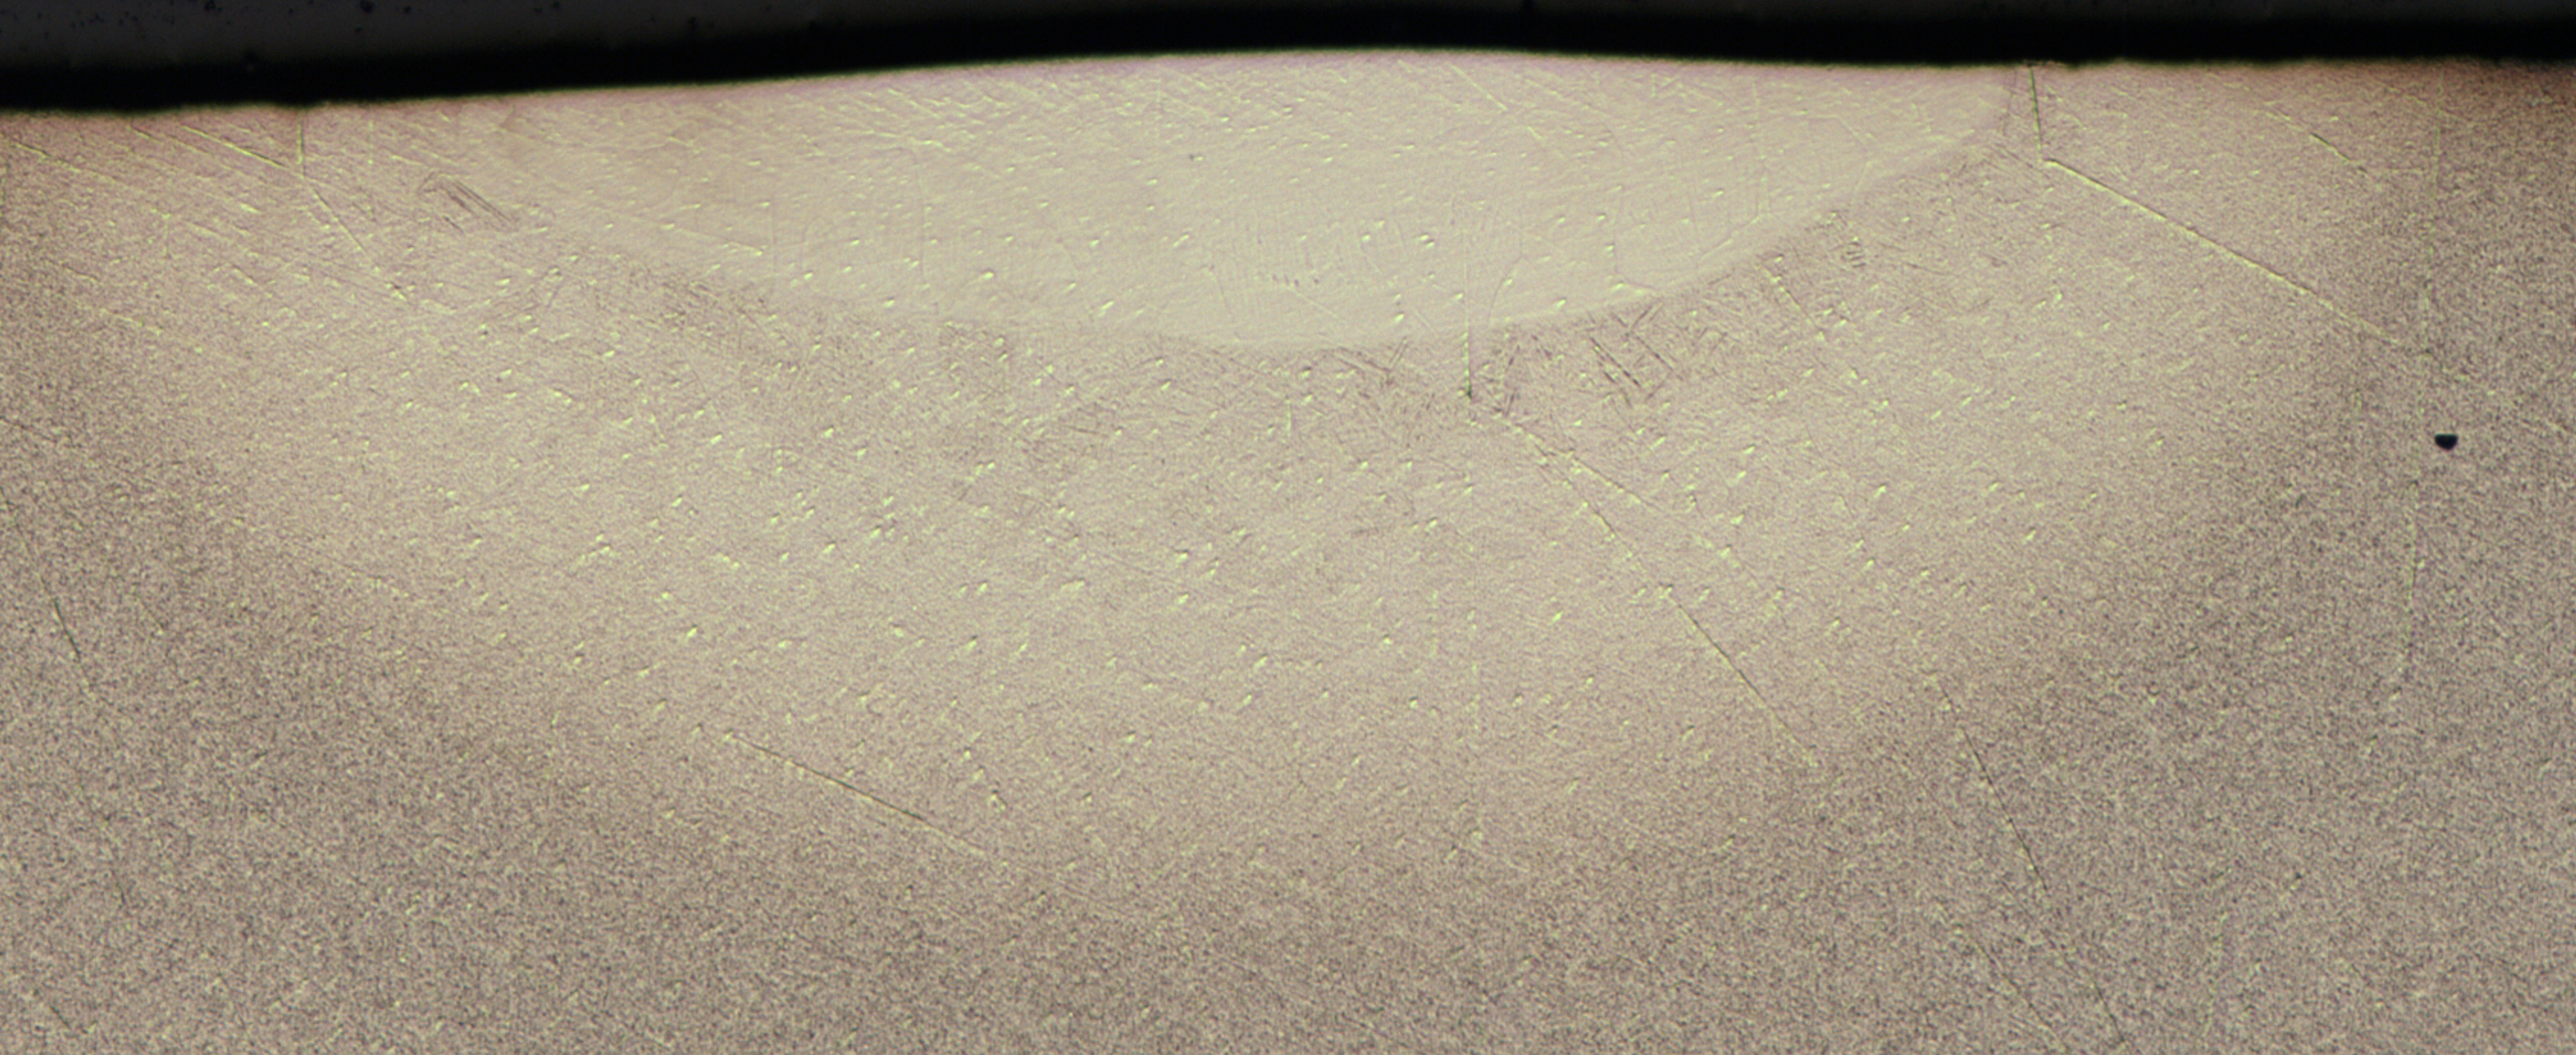
\includegraphics[width=\textwidth]{melt_track_image}
		\caption{Sample image of the etched slice}
		\label{fig:melt_track_image}
		\end{subfigure}
			\begin{subfigure}{0.495\textwidth}
			\includegraphics[width=\textwidth]{melt_track_bitmap}
			\caption{Melt pool extracted from etched slice}
			\label{fig:melt_track_bitmap}
			\end{subfigure}
	\caption{Analysis of sliced sample in Ti-64 validation}
	\label{fig:melt_track}
\end{figure}
The experiment and simulation were compared and the resulting error for the width can be seen in Figure \ref{fig:ti64_melt_track_width} and the depth can be seen in Figure \ref{fig:ti64_melt_track_depth}.
\begin{figure}[!htb]\centering
	\begin{subfigure}[c]{0.45\textwidth}\centering
	\includegraphics[width=\textwidth]{ti64_melt_track_width}
	\caption{Width}
	\label{fig:ti64_melt_track_width}
	\end{subfigure}\hfill{}
		\begin{subfigure}[c]{0.45\textwidth}\centering
		\includegraphics[width=\textwidth]{ti64_melt_track_depth}
		\caption{Depth}
		\label{fig:ti64_melt_track_depth}
		\end{subfigure}
	\caption{Comparison of simulation and experimentation in Ti-64 validation.}
	\label{fig:ti64_melt_track}
\end{figure}
The average values which are reported on the graph have an associated standard deviation of the 0.62 $\mu m$, 13.7 $\mu m$, and 7.74 $\mu m$ for the width measurements for the energy densities of 15 $\frac{W}{mm^3/sec}$, 18 $\frac{W}{mm^3/sec}$, and 24 $\frac{W}{mm^3/sec}$ respectively.  For the track depth the standard deviations are 70.2 $\mu m$, 113.7 $\mu m$, and 13.7 $\mu m$ for the energy densities of 15 $\frac{W}{mm^3/sec}$, 18 $\frac{W}{mm^3/sec}$, and 24 $\frac{W}{mm^3/sec}$ respectively.

From the plots, it can be seen that the simulation is capable of predicting the width within 3\% error and the depth error is between 15\% and 25\%.  The error in the width is very acceptable at less than 3\%.
However, the error in the depth is larger due to the resolution (voxel size) of the simulation chosen and its relative size to the depth.  This error, of approximately 20\%, for the depths which range from 450-500 $\mu m$ is 1.3-1.7 times the resolution, 60 $\mu m$, of the simulation.  Since the trends of the simulation and experimentation match and the error is within two resolution distances the 20\% error in the depth is considered acceptable as well. 
This shows that the mathematical models developed are accurate and if the material property is well characterized, the simulation will produce accurate results.


	% \FloatBarrier

\section{Tuning algorithm implementation}
	
	% One research question you may explore:  how many unknown parameters can your approach handle and what are the errors when increasing the number of unknowns? 
	\subsection{Tuning algorithm description}
	\label{algrothim_description}

The search algorithm chosen was the Nelder-Mead search algorithm \cite{nelder_1965}.  This method was selected because it is one of the most popular direct search methods for the minimization of functions.  The Nelder-Mead approach is a local optimization search which does not rely on knowledge of the gradient to select the next search point.  This is critical for the application to simulation results because the gradient is unknown and finding it would involve running a large number of simulations.  With simulation times that can reach into days long, this is a critical consideration.  
Instead of knowing the actual function, it relies on n+1 vertices.  This results in a smaller number of simulation runs being needed to perform the minimization \cite{wang_2011}.
The flow chart in Figure \ref{fig:nm_flow} is the flow which is used to determine the next search point.
\begin{figure}[!htb]
	\centering
	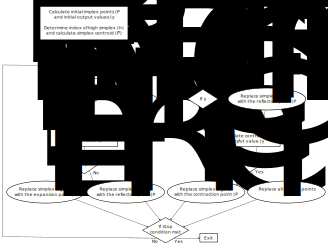
\includegraphics[width=\textwidth]{nm_flow}
	\caption{Flow chart for the Nelder-Mead search algorithm\cite{nelder_1965}}
	\label{fig:nm_flow}
\end{figure}

The search begins by calculating the reflection point using Equation \ref{eqn:reflection} where $\alpha$ is the reflection coefficient.
	\begin{equation}\label{eqn:reflection}
		P_{refl} = (1 + \alpha) P_{cent} - \alpha P_{high}
	\end{equation}
If this reflection point is smaller than the smallest current simplex value, then the expansion is calculated using Equation \ref{eqn:expansion}, where $\gamma$ is the expansion coefficient.
	\begin{equation}\label{eqn:expansion}
		P_{exp} = \gamma P_{refl} - (1 - \gamma) P_{center}
	\end{equation}
If the expansion point is smaller than the reflection point, then the expansion point is used to replace the largest simplex member.  Otherwise, if the reflection point is larger than the expansion point, the reflection point is used to replace the largest member of the simplex, and the algorithm is restarted.
If the reflection point is larger than the smallest simplex point and smaller than the second largest point, then the highest point of the simplex is replaced with the reflection and the algorithm is restarted. 
If the reflection point is between the simplex highest value and second highest value, a contraction is calculated, using Equation \ref{eqn:reflection}, with the highest values being replaced with the reflection.  Otherwise the contraction is calculated with the original simplex still using Equation \ref{eqn:reflection}, where $\beta$ is the contraction coefficient.
	\begin{equation}\label{eqn:contraction}
		P_{cont} = \beta P_{high} - (1 - \beta) P_{cent}	
	\end{equation}
If the contraction point is smaller than the largest point of the simplex, then the contraction replaces the largest point and the algorithm is continued.
However, if the contraction point is larger than the highest point, a shrink step is performed, detailed in Equation \ref{eqn:shrink}, where $\delta$ is the shrink coefficient and the algorithm is restarted.
	\begin{equation}\label{eqn:shrink}
		P_{i} = \delta P_{i} + (1 - \delta) P_{low}
	\end{equation}

	\subsection{Selection of Properties}
	\label{sensetivity_results}

In order to reduce the complexity of the search algorithm, a sensitivity analysis was performed in \ref{OTHERPAPER}.
This work began by finding the material properties which were needed in the models these can be seen in Table \ref{tab:sens_properties}.
\begin{table}[!htb]
	\centering
	\caption{Key material properties in thermal modeling of AM}
	\label{tab:sens_properties}
	\begin{tabular}{|c|c|} \hline
		Material Property & Reference \\ \hline
		Solidus temperature & 
			\begin{tabular}{c}
				\cite{joseph_r_davis_aluminum_2001},
				\cite{lundberg_material_1994},  \\
				\cite{ulbrich_wire_2014},
				\cite{matweb}
			\end{tabular}\\ \hline
		Liquidus temperature & 
			\begin{tabular}{c}
				\cite{joseph_r_davis_aluminum_2001}, 
				\cite{lundberg_material_1994}, \\
				\cite{ulbrich_wire_2014}, 
				\cite{matweb}
			\end{tabular}\\ \hline
		Solid density & 
			\begin{tabular}{c}
				\cite{matweb},
				\cite{amesweb}
			\end{tabular}\\ \hline
		Fluid density & 
			\begin{tabular}{c}
				\cite{matweb},
				\cite{schmitz_density_2012},\\
				\cite{leitner_thermophysical_2017}
			\end{tabular}\\ \hline
		Specific heat & 
			\begin{tabular}{c}
				\cite{lundberg_material_1994},
				\cite{leitner_thermophysical_2017}
			\end{tabular}\\ \hline
		Thermal conductivity & 
			\begin{tabular}{c}
				\cite{lundberg_material_1994},
				\cite{leitner_thermophysical_2017}
			\end{tabular}\\ \hline
		Absorptivity & 
			\begin{tabular}{c}
				\cite{funck_tailored_2014},
				\cite{boyden_temperature_2006},\\
				\cite{el-hameed_anodic_2017}
			\end{tabular}\\ \hline
	\end{tabular}
\end{table}

These properties were varied according to a Placket-Burman design of experiment in order to determine the properties which, when changed, had a statically significant effect on the resulting melt pool width, depth, and volume, as measured in Figure \ref{fig:slices}.
\begin{figure}[!tb]\centering
	\begin{subfigure}[t]{0.22\textwidth}\centering
	\includegraphics[height=0.6in]{slice_y_annotated}
	\caption{Width}
	\label{fig:slice_y_annotated}
	\end{subfigure}
		\begin{subfigure}[t]{0.77\textwidth}\centering
		\includegraphics[height=0.6in]{slice_x_annotated}
		\caption{Length}
		\label{fig:slice_x_annotated}
		\end{subfigure}
	\caption{Example measurements of the melt pool}
	\label{fig:slices}
\end{figure}
Analyzing these results with Pareto charts of the standardized effects of the variables and partial regression plots of the residuals it was determined that the variables in Table \ref{tab:crit_mat_prop}.
\begin{table}[!htb]
	\centering
	\caption{Critical material properties}
	\label{tab:crit_mat_prop}
		\begin{tabular}{|c|} \hline 
			Laser absorption at 880\degree C \\ \hline
			Laser absorption at 922\degree C \\ \hline
			Thermal conductivity at 922\degree C \\ \hline
			Thermal conductivity at 1491\degree C \\ \hline
			Specific heat at 733\degree C \\ \hline
		\end{tabular}
\end{table}
This work only focused on the material properties and the laser diameter was included due to the difficulty associated with accurately measuring the diameter.


	\subsection{Tuning and Simulation setup}
	\label{sim_setup}

For this study, the Nelder Mead search algorithm parameters which were used can be seen in Table \ref{tab:nm_parameters}.
\begin{table}[!htb]
	\centering
	\caption{Nelder-Mead algorithm parameters}
	\label{tab:nm_parameters}
		\begin{tabular}{|c|c|} \hline 
			Parameter & Value \\ \hline
			$\alpha$ & 5.0 \\ \hline
			$\gamma$ & 10.0 \\ \hline
			$\beta$ & 0.5 \\ \hline
			$\sigma$ & 0.5 \\ \hline
		\end{tabular}
\end{table}
These parameters were chosen because they fell within the guidelines from the algorithm description and after trial and error produced the most efficient tuning \cite{nelder_1965}.

The starting values which were used as the starting point for the search algorithm can be seen in Table \ref{tab:starting_mat_prop_complete}.  These values were chosen based on the values which were found in literature for similar aluminum alloys.  The laser diameter which was chosen based on the measuring of a melt track width on a substrate. 
\begin{table}[!htb]
	\centering
	\caption{Material properties found in literature}
	\label{tab:starting_mat_prop_complete}
		\begin{tabular}{|c|c|c|c|} \hline 
			Property & Material Temp. & Value & Ref. \\ \hline
			Laser absorption & 880\degree C & 15.0\% & \cite{boyden_temperature_2006} \\ \hline
			Laser absorption & 922\degree C & 30.0\% & \cite{boyden_temperature_2006} \\ \hline
			Thermal conductivity & 922\degree C & 88.8 $\frac{W}{mK}$ & \cite{leitner_thermophysical_2017}\\ \hline
			Thermal conductivity & 1491\degree C & 104.9 $\frac{W}{mK}$ & \cite{leitner_thermophysical_2017}\\ \hline
			Specific heat & 733\degree C & 1108.0 $\frac{J}{kgK}$ & \cite{leitner_thermophysical_2017}\\ \hline
			Laser diameter & & 1.6 mm & \\ \hline
		\end{tabular}
\end{table}

The experimental setup which was used as a simple laser scanning of the surface of a substrate, as shown in Figure \ref{fig:melt_validation_example}, with the parameters shown in Table \ref{tab:exp_constants}.  This was chosen in order to simplify the experiment.  This setup removes the complexity associated with adding material including the rate of material addition, molten metal flow parameters, and acceleration effect associated with turning during deposits.
\begin{figure}[!htb]
	\centering
	\includegraphics[width=0.75\textwidth]{melt_validation_example}
	\caption{Example of simulation setup used to determine melt track size}
	\label{fig:melt_validation_example}
\end{figure}
\begin{table}[!htb]
	\centering
	\caption{Experimental constants used in tuning experiments}
	\label{tab:exp_constants}
	\begin{tabular}{|l|l|} \hline
		Parameter & Value \\ \hline
% 			Material & NEED TO LOOK UP \\ \hline
		Resolution & 100 $\mu m$ \\ \hline
		Laser Power & 1,750 W \\ \hline
		Laser Scan Speed & 1143 mm/min \\ \hline
		Laser Profile & Top Hat \\ \hline
		Scan Length & 77 mm \\ \hline
		Substrate dimensions & 82 mm x 8 mm x 8 mm \\ \hline
	\end{tabular}
\end{table}




	\subsection{Simulation analysis}
	\label{sim_analysis}

Upon completion of each simulation run, the saved data files were analyzed to determine the regions of the simulation that had melted.  This was done by developing a map that marked the locations of the domain that had ever been in the fluid phase.  This map was then used to determine the width and depth of the melt track along the scan length, excluding the beginning and end where effects from starting and stopping motion would affect the results.  These width and depth measurements along the scan length were averaged to develop a single measurement that could be compared to experimentation.  

The experimental results were similarly determined, however instead of a continuous set of measurements, there were 4 discrete measurements.  These were obtained by slicing the substrate at the prescribed locations using a wire \ac{EDM}.  These slices were polished using an automatic polishing machine up to a mirror finish and etched using Keller's reagent to make the microstructural differences visible by an optical microscope, an example of this can be seen in Figure \ref{fig:7075_7_8C}, where the dark region had been melted during the experimentation.
\begin{figure}[!htb]
	\centering
	\includegraphics[width=0.5\textwidth]{7075_7_8C}
	\caption{Example of sliced, polished, and etched slice from Aluminum experimentation}
	\label{fig:7075_7_8C}
\end{figure}

For the Nelder-Mead search to function properly, a response variable needed to be defined.  This function needed to characterize the accuracy of the simulation into a single parameter which could be minimized and upon minimization would result in the most accurate simulation.  To accomplish this goal, Equation \ref{eqn:response} was developed.  This equation takes into account the error in the width of the simulation along with the error in the depth.  This equation results in a non-negative number where 0 represents a simulation that perfectly matched experimentation.

\begin{equation}\label{eqn:response}
	\begin{split}
		Response =  \Biggl ( &\frac{\lvert Sim.\ Width - Exp.\ Width \rvert}{Exp.\ Width} + \\ 
		&\frac{\lvert Sim.\ Depth - Exp.\ Depth \rvert}{Exp.\ Depth} \Biggr ) * 100
	\end{split}
\end{equation}
	% \FloatBarrier

\section{Results}
	\subsection{Search algorithm results}
	\label{results}

The search algorithm was allowed to search the space to determine the best material properties.  The resulting response variables can be found in Figure \ref{fig:response_complete}.  Where the blue circular markers indicate material datasets which developed a melt track and the red diamond markers did not have the energy density to produce a melt track.
\begin{figure}[!htb]
	\centering
	\includegraphics[width=0.75\textwidth]{response_complete}
	\caption{Response variable of the search algorithm for material properties and laser diameter}
	\label{fig:response_complete}
\end{figure}
Due to the vast difference in scales of the initial responses and the final response variables, a new plot was created which has a max Y value of just over 30.  In this plot the blue circular markers are ones which have a response variable less than 30, the green triangle markers are those which completed with a melt track but had response variables greater than 30, and the red diamond markers are those which did not produce a melt track.
\begin{figure}[!htb]
	\centering
	\includegraphics[width=0.75\textwidth]{response_zoomed}
	\caption{Response variable of the search algorithm for material properties and laser diameter with max y axis value of 30}
	\label{fig:response_zoomed}
\end{figure}
In addition to these plots the error in the width and depth were plotted and can be seen in Figure \ref{fig:tuning_error_complete}.  In these plots, it can be seen that the error in the width is 8.83\% and the error in the depth is 0.03\%.  It is not fully understood why all the error is coming from the width, however it is theorized that this is a product of the difference in the size of the width vs the depth since the width is nearly triple that of the depth.
\begin{figure}[!htb]\centering
	\begin{subfigure}[c]{0.475\textwidth}\centering
	\includegraphics[width=\textwidth]{tuning_error_depth_complete}
	\caption{Melt track depth}
	\label{fig:tuning_error_depth_complete}
	\end{subfigure}\hfill{}
		\begin{subfigure}[c]{0.475\textwidth}\centering
		\includegraphics[width=\textwidth]{tuning_error_width_complete}
		\caption{Melt track width}
		\label{fig:tuning_error_width_complete}
		\end{subfigure}
	\caption{Error in the individual runs of the simulations during the tuning algorithm}
	\label{fig:tuning_error_complete}
\end{figure}

The search algorithm completed and reduced the combined error from over 600\% when starting from the material properties found in literature for the generic aluminum material properties, found in Table \ref{tab:starting_mat_prop_complete}, to 9.1\% when using the values found in Table \ref{tab:7000_mat_prop_complete}.
\begin{table}[!htb]
	\centering
	\caption{Optimized material properties and laser diameter dataset for the developed simulation}
	\label{tab:7000_mat_prop_complete}
		\begin{tabular}{|c|c|c|} \hline 
			Property & Material Temp. & Value \\ \hline
			Laser absorption & 880\degree C & 16.8\% \\ \hline
			Laser absorption & 922\degree C & 10.0\%\\ \hline
			Thermal conductivity & 922\degree C & 32.2 $\frac{W}{mK}$\\ \hline
			Thermal conductivity & 1491\degree C & 152.3 $\frac{W}{mK}$\\ \hline
			Specific heat & 733\degree C & 2957.6 $\frac{J}{kgK}$ \\ \hline
			Laser diameter & & 0.864 mm \\ \hline
		\end{tabular}
\end{table}

	\subsection{Search results validation}
	\label{validation}

In order to ensure that the search algorithm results were valid across laser travel speeds and power levels, a range of 8 other parameters were compared with experimental results.
These experiments and simulations were the setup and analyzed as was used for the tuning experimental setup.  The base experimental parameters can be seen in Table \ref{tab:exp_constants} with the scan speed and laser power being varied as seen in Table \ref{tab:val_parameters} and the simulation material properties were used from Table \ref{tab:7000_mat_prop_complete}.
\begin{table}[!htb]
	\centering
	\caption{Validation processing parameters}
	\label{tab:val_parameters}
		\begin{tabular}{|c|c|c|} \hline 
			Exp. Id. & Scan speed (mm/min) & Laser Power (W) \\ \hline
			1 & 762 & 1000 \\ \hline  % 0
			2 & 762 & 1500 \\ \hline  % 1
			3 & 762 & 1250 \\ \hline  % 2
			4 & 1143 & 1250 \\ \hline % 3
			5 & 1143 & 1500 \\ \hline  % 5
			6 & 1524 & 1750 \\ \hline  % 6
			7 & 1524 & 1500 \\ \hline  % 7
			8 & 1524 & 2000 \\ \hline  % 8
		\end{tabular}
\end{table}
The exerimental result were collected and graphed in Figure \ref{fig:melt_track_val} and \ref{fig:melt_track_val_baseline} as the red dashed line and were used as the ground truth with which the models were compared.

These speeds and powers were first completed with the literature determined values from Table \ref{tab:starting_mat_prop_complete} and the results can be seen in Figure \ref{fig:melt_track_val_baseline}.
\begin{figure}[!htb]\centering
	\begin{subfigure}[c]{0.45\textwidth}\centering
	\includegraphics[width=\textwidth]{melt_track_val_baseline_depth}
	\caption{Melt track depth}
	\label{fig:melt_track_val_baseline_depth}
	\end{subfigure}\hfill{}
		\begin{subfigure}[c]{0.45\textwidth}\centering
		\includegraphics[width=\textwidth]{melt_track_val_baseline_width}
		\caption{Melt track width}
		\label{fig:melt_track_val_baseline_width}
		\end{subfigure}
	\caption{Comparison of experimental and simulated results for validation points with generic literature values for material dataset}
	\label{fig:melt_track_val_baseline}
\end{figure}
Where the red dashed line is the experimental results, the blue dots are the simulation predictions, and the green line is the error when comparing the simulated results to the experimental results.
These results show that over the 9 initial parameter sets, when a melt track was developed, the average absolute value of the error in the depth was approximately 290\% and the average error in the width was approximately 265\%.  To put this into terms of the response variable of the search algorithm, the sum of the width and depth error, would be 555\% combined error.
Additionally, run 1 was unable to develop a melt pool, which is contrary to the experiments where all the parameter sets had a stable melt track.  These results corroborate the results from Figure \ref{fig:response_complete} which showed that the parameter set used for tuning initial dataset of material properties found in the literature is wholly inadequate for simulating the process at hand. 

In contrast to these results, the material dataset which was found in Table \ref{tab:7000_mat_prop_complete} was used to simulate each parameter set, and the results can be seen in Figure \ref{fig:melt_track_val}.
\begin{figure}[!htb]\centering
	\begin{subfigure}[c]{0.45\textwidth}\centering
	\includegraphics[width=\textwidth]{melt_track_val_depth}
	\caption{Melt track depth}
	\label{fig:melt_track_val_depth}
	\end{subfigure}\hfill{}
		\begin{subfigure}[c]{0.45\textwidth}\centering
		\includegraphics[width=\textwidth]{melt_track_val_width}
		\caption{Melt track width}
		\label{fig:melt_track_val_width}
		\end{subfigure}
	\caption{Comparison of experimental and simulated results for validation points with optimized values for material dataset}
	\label{fig:melt_track_val}
\end{figure}
Where the red dashed line is the experimental results, the blue dots are the simulation predictions, and the green line is the error when comparing the simulated results to the experimental results.
These results show the average error in the width was approximately 17\% and the average error in the depth was approximately 5\%, which creates a combined error of only 22\%.  These results show that the optimized dataset is better at predicting the combined error of the simulation by over 500\%.  This results in a simulation which can be leveraged more intensely during the process development and build qualification process.  
These results are from a wide parameter set which encompasses most of the usable parameter space for deposition found experimentally.  This improvement in accuracy will allow for a greater application in the model in the determination of an optimized parameter set for a given build.  In addition, the model is seen to be more accurate at parameters above the parameter used during the optimization.  This leads to the conclusion that if a more accurate simulation is needed, the optimization should be done at a parameter set near the desired parameter set.

	
	% For validation and demonstration, you might like to find a material with existing known parameters.  You can then use your approach to find one parameter that pretend to be unknown, such as thermal conductivity coefficient, etc.  Then you can compare the known parameter value with your calculation.  If successful, you can use two parameters that pretend to be unknown …
% \FloatBarrier

\section{Conclusions}
\label{conclusions}

This work shows that the Nelder-Mead search algorithm is an appropriate multidimensional search algorithm for the determination of the optimal dataset for improved simulation accuracy.  It was capable of reducing the simulated melt track depth and width of a set of processing parameters by over 500\%, as shown in Figures \ref{fig:melt_track_val_baseline} and Figure \ref{fig:melt_track_val}, which used datasets from literature (Table \ref{tab:starting_mat_prop_complete}) and the optimized dataset (Table \ref{tab:7000_mat_prop_complete}) respectively.  This was done by defining the response variable (Equation \ref{eqn:response}) for the search algorithm to be the sum of the error in the width and the depth, which facilitated an efficient search.  
This methodology can be used to develop accurate simulations for any material which is not well published or to increase the accuracy of a simulation which utilizes approximations of first principles in order to increase its efficiency.


% \section{Declarations}
% \begin{description}
	% \item[Funding:] This project was supported by National Science Foundation Grants CMMI 1625736 and EEC 1937128, Product Innovation and Engineering through Navy STTR project Contract \#N6833520C0029, and the Intelligent Systems Center at Missouri S\&T,  Their financial support is greatly appreciated.
	% \item[Financial interests:] All authors declare they have no financial interests.
	% \item[Data Availability:] All data generated or analysed during this study are included in this published article.
% \end{description}


\bibliography{references.bib}

\end{document}
